\documentclass[12 pt, a4paper]{article}
\usepackage{amsmath, latexsym}
\usepackage{amsmath, amssymb}
\usepackage{amsopn}
\usepackage{float}
\usepackage{placeins}
\usepackage{mathrsfs}
\usepackage{amssymb}
\usepackage{enumerate}
\usepackage{paralist}
\usepackage{enumitem}
\usepackage{lipsum}
\usepackage{multirow}
\usepackage{multicol}
\usepackage[pdftex]{graphicx}
\usepackage[pdftex]{hyperref}
\usepackage{scalefnt}
\usepackage{setspace}
\usepackage{charter}
\usepackage{epsfig}
\usepackage{subfigure}
\usepackage{array,arydshln}
\usepackage{enumerate}
\usepackage{amsthm}
\usepackage{graphicx}
\usepackage{color,soul}
\usepackage{enumitem}
\usepackage{tcolorbox}
\usepackage{tikz}
\usetikzlibrary{arrows}
\usepackage{verbatim}
\usepackage{tabularx}
\usepackage[super]{nth}
\newtheorem{prop}{Proposition}
\newtheorem{thm}{Theorem}
\newtheorem{cor}[thm]{Corollary}
\newtheorem{lemma}[thm]{Lemma}
\newtheorem{remark}{Remark}
\usepackage{array}
\newtheorem{theorem}{Theorem}
%\theoremstyle{definition}
%\newtheorem{definition}{Definition}[section]
\newtheorem{definition}{Definition}
\usepackage{algorithm}
%\usepackage{algpseudocode}
\usepackage{algorithmic}
%%%%%%%%%%%%%%%%%%%%%%%%%%%%%%%%%%%%%%%
\usepackage{mathtools}
\usepackage{amsthm}
\usepackage{amsmath,amsfonts}
\usepackage{amssymb}
\usepackage[round]{natbib}
\setcitestyle{square}
\renewcommand{\sp}[1]{{ \text{Reg}(#1)}}
\def\I{{\mathcal I}}
\def\J{{\mathcal J}}
%\usepackage{stackengine}

%%%%%%%%%%%%%%%%%%%%%%%%%%%%%%%%%%%
\makeatletter
\def\BState{\State\hskip-\ALG@thistlm}
\makeatother

\newcommand{\HRule}{\rule{\linewidth}{1mm}}
\topmargin = -30 mm
\textwidth = 175 mm
\textheight = 270 mm
\oddsidemargin = -10 mm
\evensidemargin = -10 mm

\setlist[description]{font=\itshape}
\begin{document}
    \pagestyle{empty}
\vskip 0.2cm
    \begin{tabular}{l c}
        \multirow{0}{*}
        {
\includegraphics[scale=0.50]{logo.jpg}}                              &
        \large\bf{INDIAN INSTITUTE OF TECHNOLOGY MANDI} \\
          \\ & \large\bf{MANDI-175075 (H.P.), INDIA} \\ & \underline{\href{www.iitmandi.ac.in}{www.iitmandi.ac.in}}
    \end{tabular}
 \vskip 0.7cm

{\raggedleft{}\HRule}
 
\begin{center}
\large\bf\underline{PROGRESS REPORT FOR THE ACADEMIC YEAR 2023}
\end{center}
\indent \textbf{Scholar's Name:} {ARJUN H KUMAR} \hfill \textbf{Roll No:} {S21008} \\
\noindent \textbf{School:} {SCEE} \hfill \textbf{Date of Registration: }{\nth{9} August 2021} \newline
\noindent \textbf{Semester:} {IV}\hfill \textbf{CGPA: }{8.57}
\newline
\noindent \textbf{Date of Last Presentation: }{\nth{29} July 2022}\hfill \textbf{Date of Current Presentation: }{x July 2023}
\\
\noindent\rule{17.69cm}{0.8pt}
   
\section{Research ~Objectives}
    
Using program analysis-
\begin{enumerate}
\item Identify various access patterns under which value-type objects should be flattened in their respective containers.
\item Build an appropriate flattening strategy for such objects in Eclipse OpenJ9 VM.
\item Improve Java applications by using static + JIT analysis based on the developed flattening strategy.
\item Explore prospective optimizations that can be enabled in JVM due to the introduction of value types.

\end{enumerate} 



\section{Introduction}

In modern object-oriented programming languages, object identity
enables fundamental features such as field mutation and synchronization. However, it also significantly affects the performance. In
particular, each distinct field access requires a memory load of the
corresponding object followed by an indirection. Several compiler
analyses and optimizations such as escape analysis and field scalar-
ization can eliminate these costs in specific scenarios; however,
such optimizations are usually limited in their scope and applica-
bility. Languages like Java allow for optimizing the access cost for
objects of certain “primitive” types; however, OO programs often
contain additional user-defined types whose objects do not depend
on an identity that is separate from their “value”. An important
development in this space has been the Project Valhalla [2], which
aims to improve the performance profile of conventional objects in
Java, and make it comparable to the performance of primitive types.
Valhalla introduces the notion of value types [4], which essentially
empowers objects to be identity-less. In order to facilitate an im-
proved performance for such objects, an important optimization
that can be performed by a value-types supporting Java Virtual
Machine (JVM) is object inlining [1] or flattening.
\clearpage
\setlist[description]{font=\itshape}
\pagestyle{empty}
\vskip 0.2cm
\begin{tabular}{l c}
	\multirow{0}{*}
	{
\includegraphics[scale=0.50]{logo.jpg}}                              &
	\large\bf{INDIAN INSTITUTE OF TECHNOLOGY MANDI} \\
	\\ & \large\bf{MANDI-175075 (H.P.), INDIA} \\ & \underline{\href{www.iitmandi.ac.in}{www.iitmandi.ac.in}}
\end{tabular}
\vskip 0.7cm
{\raggedleft{}\HRule}

\section{Work Done and Target Set for Last Year}

\subsection{Identification of value-type classes}

\subsection{Implementation in OpenJ9}



\clearpage
\setlist[description]{font=\itshape}
\pagestyle{empty}
\vskip 0.2cm
\begin{tabular}{l c}
	\multirow{0}{*}
	{
\includegraphics[scale=0.50]{logo.jpg}}                              &
	\large\bf{INDIAN INSTITUTE OF TECHNOLOGY MANDI} \\
	\\ & \large\bf{MANDI-175075 (H.P.), INDIA} \\ & \underline{\href{www.iitmandi.ac.in}{www.iitmandi.ac.in}}
\end{tabular}
\vskip 0.7cm
{\raggedleft{}\HRule}
\subsection{Changing granularity from class level to field level}

\subsection{Cache distance analysis}
\begin{figure}[h]
% \caption{Example of object inlining}
\vskip 0.2cm
\centering
% 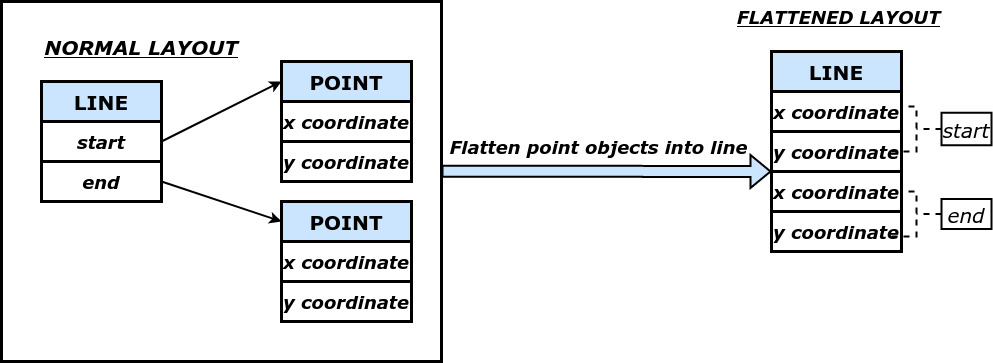
\includegraphics[scale=0.48]{Flattening_Line}
% \label{fig:Figure 1}
\end{figure}




\clearpage
\setlist[description]{font=\itshape}
\pagestyle{empty}
\vskip 0.2cm
\begin{tabular}{l c}
	\multirow{0}{*}
	{
\includegraphics[scale=0.50]{logo.jpg}}                              &
	\large\bf{INDIAN INSTITUTE OF TECHNOLOGY MANDI} \\
	\\ & \large\bf{MANDI-175075 (H.P.), INDIA} \\ & \underline{\href{www.iitmandi.ac.in}{www.iitmandi.ac.in}}
\end{tabular}
\vskip 0.7cm
{\raggedleft{}\HRule}
\section{Planned Work for the Next Year}   
 \begin{enumerate}
\item Implementing a static + dynamic analysis to compute the number of distinct
		cache loads possible between two inlined field loads.

\item Evaluating the strategy over a set of standard benchmarks for JVM.

\item Preparing a manuscript describing the complete work.
 
\end{enumerate} 





\vskip 0.7cm
\section{Workshops/Conferences Attended}
\begin{enumerate}
\item International Conference on Systems, Programming, 
Languages, and Applications: Software for Humanity 
(SPLASH Companion), Virtual, December 5th-10th, 2022.
\item \nth{16} Innovations in Software Engineering Conference (ISEC), 
IIIT Allahabad, India, February 23rd-25th, 2023.
\item Software Engineering Research in India (SERI) Update Meeting, 
Goa University, India, June 2nd-3rd, 2023
\end{enumerate} 



\section{Papers Published/Communicated and Other Achievements:} 
\begin{enumerate}
\item Arjun Harikumar and Manas Thakur. “ValFinder: Finding Hidden Value-Type Classes”. 
6th Workshop on Advances in Open Runtimes and Cloud Performance Technologies (AORCPT), part of IBM WeaveSphere, Toronto, Canada, November 16th, 2022.
\end{enumerate} 


\clearpage
\setlist[description]{font=\itshape}
\pagestyle{empty}
\vskip 0.2cm
\begin{tabular}{l c}
	\multirow{0}{*}
	{
\includegraphics[scale=0.50]{logo.jpg}}                              &
	\large\bf{INDIAN INSTITUTE OF TECHNOLOGY MANDI} \\
	\\ & \large\bf{MANDI-175075 (H.P.), INDIA} \\ & \underline{\href{www.iitmandi.ac.in}{www.iitmandi.ac.in}}
\end{tabular}
\vskip 0.7cm
{\raggedleft{}\HRule}


\bibliographystyle{plainnat}
\bibliography{biblography}
     
\clearpage
\setlist[description]{font=\itshape}

	\pagestyle{empty}
	\vskip 0.2cm
	\begin{tabular}{l c}
		\multirow{0}{*}
		{
\includegraphics[scale=0.50]{logo.jpg}}                              &
		\large\bf{INDIAN INSTITUTE OF TECHNOLOGY MANDI} \\
		\\ & \large\bf{MANDI-175075 (H.P.), INDIA} \\ & \underline{\href{www.iitmandi.ac.in}{www.iitmandi.ac.in}}
	\end{tabular}
	\vskip 0.7cm
	
	{\raggedleft{}\HRule}
	\begin{center}
	\large\bf{\underline{REPORT BY APC/DC COMMITTEE}} 
	\end{center}

\begin{enumerate}
    \item \textbf{Has the student met the targets set for last year?}
    \vskip 0.2cm
	\textbf{(a) Mention the Achieved Targets:}
	
	\begin{itemize}
	    \item 
	    \item 
	\end{itemize}
	\textbf{(b) If not what are the major reasons?}
	\vskip 0.2cm
	\hskip 0.7 cm N/A
	\vspace{0.2cm}
	\item \textbf{Is there a reasonable target set for next year? Give detailed plan.}
% 	\vspace*{1.0 cm}
	\begin{figure}[h]
    % \vskip 0.2cm
    \centering  
    % 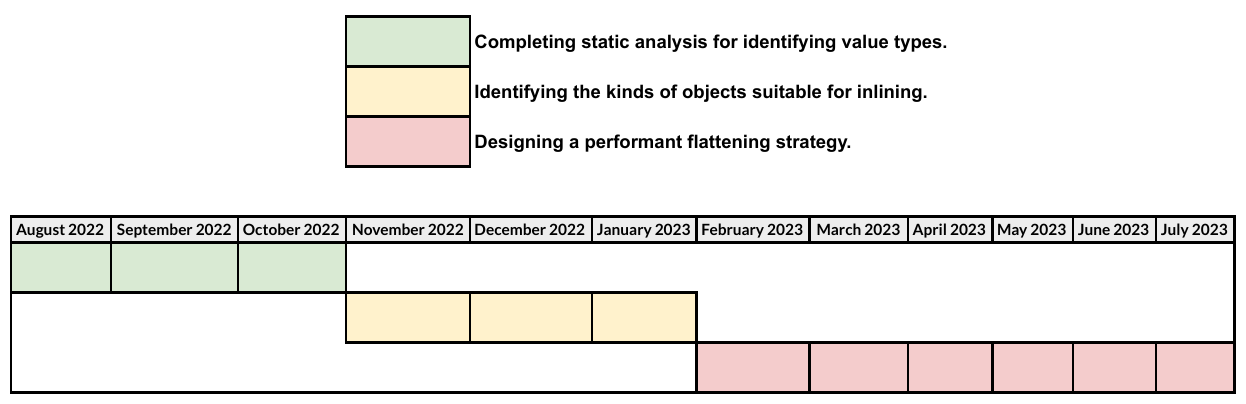
\includegraphics[scale=0.4]{Gantt_Chart.png}
    \end{figure}
	\item \textbf{What is the perception of the student and guide(s) about the fraction of thesis work completed?}
	\vskip 0.2cm
	\hskip 0.7 cm \text{N/A}
	\item\textbf{What is the approximate time scale for thesis submission (only for students in their
		\bf \nth{5} year or above for Ph.D. and \nth{3} year and above for M.S. students).}
	\vskip 0.2cm
	\hskip 0.7 cm N/A
	\item\bf{Any other observations of the committee.}
	\vspace*{1.0 cm}


\end{enumerate}
\clearpage
\setlist[description]{font=\itshape}
\pagestyle{empty}
\vskip 0.2cm
\begin{tabular}{l c}
	\multirow{0}{*}
	{
\includegraphics[scale=0.50]{logo.jpg}}                              &
	\large\bf{INDIAN INSTITUTE OF TECHNOLOGY MANDI} \\
	\\ & \large\bf{MANDI-175075 (H.P.), INDIA} \\ & \underline{\href{www.iitmandi.ac.in}{www.iitmandi.ac.in}}
\end{tabular}
\vskip 0.7cm
{\raggedleft{}\HRule}
\textbf{Recommendation of APC/DC} \textit{(Tick Appropriately)}
\begin{enumerate}
	\item
	\begin{enumerate}
\item Continuation of Registration is \textbf{Recommended/ Not Recommended.}
\item Continuation of Scholarship/Research Assistantship \textbf{ Recommended/ Not Recommended.}
\item Enhancement of Scholarship from JRF to SRF is \textbf{Recommended/ Not Recommended } (only
after Two Year of Registration).
\end{enumerate}
\item
\textbf{Source of Funding/Scholarship:}

\item \textbf{OVERALL PERFORMANCE: Very Good/Good/Satisfactory/Unsatisfactory}
\item \textbf{Any Other Recommendation/Comments} \textit{(Attach separate sheet).}
Same as the above observation.
\end{enumerate}
\vspace*{1cm}

\noindent \textbf{COMMITTEE MEMBERS}\\\\
\indent
\begin{tabular}{|p{1.25cm}|p{5cm}|p{4cm}|p{3cm}|p{2cm}|}
	\hline\rule{0pt}{15pt} \bf S. No. & \bf Faculty Name & \bf School/Department & \bf Signature & \bf Remarks \\ 
	\hline\rule{0pt}{18pt}\bf 1. & Dr. A.D. Dileep  & SCEE &  &  \\[10pt]
	\hline\rule{0pt}{18pt}\bf 2. & Dr. Aditya Nigam & SCEE &  &  \\ [10pt]
	\hline \rule{0pt}{18pt}\bf3. & Dr. Gaurav Bhutani & SCEE &  &  \\ [10pt] 
	\hline \rule{0pt}{18pt}\bf4. & Dr. Manas Thakur & SCEE &  &  \\ [10pt] 
	\hline \rule{0pt}{18pt}\bf5. & Dr. Varunkumar Jayapaul & SCEE &  &  \\ [10pt]
	\hline 
\end{tabular} \\\\\\\\
\textbf{Signature of the Supervisor} \hspace{7.0cm} \textbf{School Chairperson}\\
Date: \hspace{11.3cm}  Date:\\
\vspace{1cm} \\
\hspace*{6cm}\textbf{Associate Dean (Research)}\\
\hspace*{6cm}Date:\\\\
\textbf{Note:}

\begin{enumerate}[label=(\roman*)]
	\item Ph.D. Scholar shall, after Registration, submit a written report to Doctoral Committee in the required
	format, annually for the first three years, and every six months thereafter.
	\item M.S. Scholar shall, after Registration, submit annually a written report to Academic Progress Committee.
	\item Attach additional sheets if required.
\end{enumerate}



\clearpage
\setlist[description]{font=\itshape}
\pagestyle{empty}
\vskip 0.2cm
\begin{tabular}{l c}
	\multirow{0}{*}
	{
\includegraphics[scale=0.50]{logo.jpg}}                              &
	\large\bf{INDIAN INSTITUTE OF TECHNOLOGY MANDI} \\
	\\ & \large\bf{MANDI-175075 (H.P.), INDIA} \\ & \underline{\href{www.iitmandi.ac.in}{www.iitmandi.ac.in}}
\end{tabular}
\vskip 0.7cm
{\raggedleft{}\HRule}

\begin{center}
	\large\bf{\underline{APC/DC RECOMMENDATION (Part B)}} 
\end{center}


\noindent  \textbf{Scholar's Name:} {ARJUN H KUMAR} \hfill \textbf{Roll No:} {S21008} \\
\noindent \textbf{School:} {SCEE} \hfill \textbf{Date of APC/DC meeting: }{X July 2022}
\vskip 0.5cm
\noindent \begin{tabular}{|p{4.2cm}|p{5cm}|p{7cm}|}
\hline\rule{0pt}{5pt} \bf  & \centering \textbf{Performance} \centering \newline(Poor, Average, Good, Very good, Exceptional)  & \hspace{2.5cm}\bf Suggestions  \\[5pt] 
\hline\rule{0pt}{5pt} \begin{center} \bf Oral Communication and Presentation \end{center} &   &   \\[5pt]
\hline\rule{0pt}{5pt} \begin{center} \bf Subject Knowledge \end{center} &   &   \\[5pt]
\hline\rule{0pt}{5pt} \begin{center} \bf Research Output \end{center} &   &   \\[5pt]
\hline \multicolumn{3}{|c|}{{\multirow{1.5}{*}{ \textbf{OVERALL PERFORMANCE \textit{(as per Part-A): Very Good/Good/Satisfactory/Unsatisfactory:}}} 
} } \\
\multicolumn{3}{|c|}{}                  \\
\multicolumn{3}{|c|}{}                  \\

\hline \multicolumn{3}{|c|}{{\multirow{1.5}{*}{ \textbf{Overall feedback/Remarks:} } 
} } \\
\multicolumn{3}{|c|}{}                  \\
\multicolumn{3}{|c|}{}                  \\
\multicolumn{3}{|c|}{}                  \\
\hline 
\end{tabular} 
\vskip 0.7cm
\noindent\textbf{APC/Doctoral Committee}
\vskip 0.3cm

\noindent\begin{tabular}{|p{4.5cm}|p{6cm}|p{4cm}|}
	\hline\rule{0pt}{15pt} \bf  & \bf Faculty Name & \bf Signature  \\ 
	\hline\rule{0pt}{18pt}\bf Chairperson APC/DC  & Dr. Aditya Nigam  &    \\[10pt]
	\hline\rule{0pt}{18pt}\bf Guide & Dr. Manas Thakur &   \\ [10pt]
	\hline \rule{0pt}{18pt}\bf Member  & Dr. A.D. Dileep &   \\ [10pt]
	\hline \rule{0pt}{18pt}\bf Member  & Dr. Gaurav Bhutani &   \\ [10pt] 
	\hline \rule{0pt}{18pt}\bf Member  & Dr. Varunkumar Jayapaul &   \\ [10pt] 
	\hline 
\end{tabular}


%%%%%%%%%%%%%%%%%%%%%%%%%%%%%%%%%%%%%%%
%\noindent \begin{tabular}{|p{4.2cm}|p{5cm}|p{7cm}|}
%\hline\rule{0pt}{5pt} \bf  & \begin{center} \textbf{Name of the Faculty} \end{center} &  \begin{center} \textbf{Signature} \end{center} \\[5pt] 
%\hline\rule{0pt}{18pt} \begin{center} \bf Chairperson APC/DC \end{center} &  \begin{center} Dr. Samar Agnihotri \end{center} &   \\[5pt]
%\hline\rule{0pt}{18pt} \begin{center} \bf Guide
 %\end{center} &  \begin{center} Dr. Manas Thakur \end{center} &   \\[5pt]
%\hline\rule{0pt}{18pt} \begin{center} \bf Co-Guide \end{center} &  \begin{center} \end{center} &   \\[5pt]
%\hline\rule{0pt}{18pt} \begin{center} \bf Member \end{center} &  \begin{center} Dr. Gaurav Bhutani \end{center} &   \\[5pt]
%\hline\rule{0pt}{18pt} \begin{center} \bf Member \end{center} &  \begin{center} Dr. Sriram Kailasam \end{center} &   \\[5pt]
%\hline
%\end{tabular}
%%%%%%%%%%%%%%%%%%%%%%%%%%%%%%%%%%%%%%%
\vskip 0.7cm
\noindent{I have read and noted the above for compliance:}
\vskip 0.2cm
\noindent\textbf{Signature of the scholar with Date:}
\end{document}
